\documentclass{article}
\usepackage[final]{neurips_2019}
\usepackage{morris}

\makeatletter
\renewcommand{\@noticestring}{Deep Learning, Sommer 2019, Universiteit van Amsterdam}
\makeatother

\renewcommand{\thesubsubsection}{\alph{subsubsection})}

\title{Assignment 2. Recurrent Neural Networks and Graph Neural Networks}
\author{%
  Maurice Frank\\
  11650656\\
  \href{mailto:maurice.frank@posteo.de}{maurice.frank@posteo.de} \\
  Code: \href{https://github.com/morris-frank/uvadlc_practicals_2019/tree/master/assignment_2}{github}
}

\begin{document}
\maketitle

\section{Vanilla RNN versus LSTM}
\subsection{RNN derivatives}
\begin{align}
  \pf{\L}{\B{W}_{ph}}
  &= \Π \pf{}{} \· \pf{}{\B{W}_{ph}}
\end{align}
\begin{align}
  \pf{\L}{\B{W}_{hh}}
  &= \…
\end{align}

\subsection{Vanilla RNN code}
Find the code inside \texttt{vanilla\_rnn.py} and \texttt{train.py}.

\subsection{Vanilla RNN experiment}
See Figure~\ref{subsub:lstm_practice} for a overview plot of the results and Section~\ref{subsub:lstm_practice} for a discussion/comparsion of the results.

\subsection{Optimizers}

\subsection{LSTM theory}
\subsubsection{LSTM Gates}
\begin{description}
  \item[\I{input modulation gate} \(\B{g}^{(t)}\)] The input modulation gate determines candidate information from the new input (using also the old hidden state).
  We want our state values normalized but need also negative values (otherwise the cell values would only increase) which, as in this case, can be done with a \(\tanh \), squashing the input to \([-1, 1]\).
  \item[\I{input gate} \(\B{i}^{(t)}\)] The input regulates which and how much information of the input of this time step should be included in the cell and hidden state.
  As the input gate regulates the flow it is necessary to have its values bounded to \([0,1]\) which can most directly achieved by squashing the values with the sigmoid.
  \item[\I{forget gate} \(\B{f}^{(t)}\)] The forget gate regulates which and how much information from the old cell state should be disregared under the new information from the input (and the old hidden state).
  As the forget gate only changes the importance (magnitude) of the information in the cell state it should be in \([0,1]\) which is achieved with the sigmoid.
  \item[\I{output gate} \(\B{o}^{(t)}\)] The output gate regulates which and how much information from the new cell state should go into the new hidden state.
  Again its gating the values from the other tensor which is asking for a range \([0, 1]\) achieved by the sigmoid.
\end{description}

\subsubsection{Number of parameters}
We have given \(\B{x}\∈\ℝ^{T\×d}\) with \(T\) sequence length and \(d\) feature dimension.
Further we have \(n\) hidden units.
Then we have
\begin{equation*}
  4\· (d\·n + n\·n + n)
\end{equation*}
trainable parameters for \textit{one} LSTM cell.

\subsection{LSTM practice}\label{subsub:lstm_practice}
Find the code inside \texttt{lstm.py} and \texttt{train.py}.


\begin{figure}\label{fig:accuracy_loss}
  \centering
  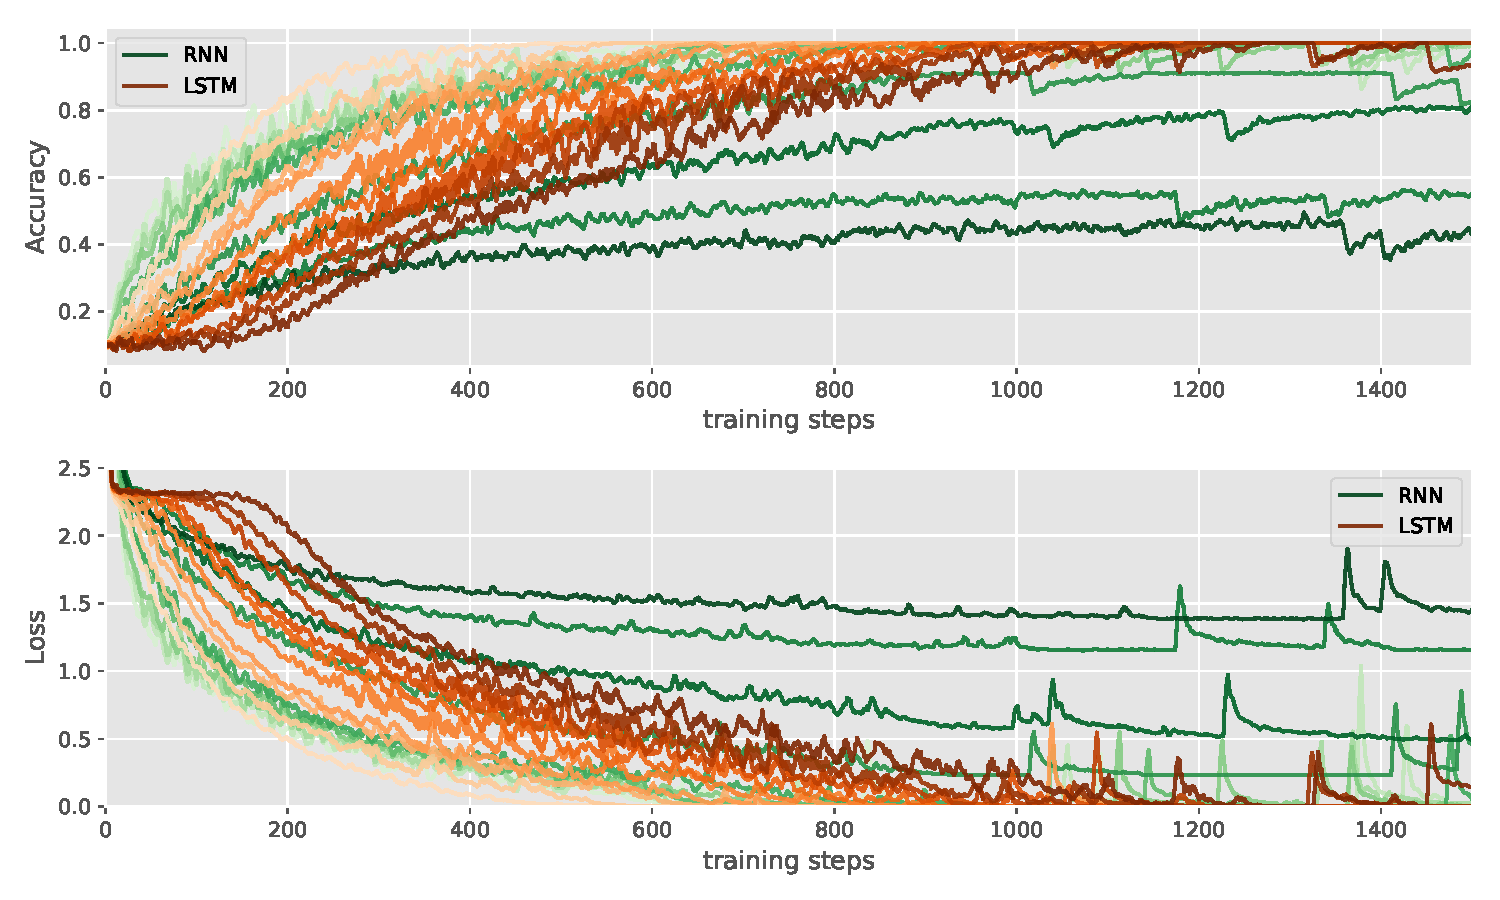
\includegraphics[width=\linewidth]{assignment_2/part1/palindrome.pdf}
  \caption{\B{Top} the accuracy and \B{bottom} the loss while training.
  Color lightness codes the palindrome length ranging from 5 numbers with the lightest color in steps of 2 to 23 numbers with the darkest color.
  (Making 9 curves per model). All curves are an average of ten runs and smoothed with a box filter of size 10 for better radibility.}
\end{figure}

\section{Recurrent Nets as Gernerative Model}
\subsection{}
\subsubsection{}
\subsubsection{}
\subsubsection{}
\subsection{}

\section{Graph Neural Networks}
\subsection{}
\subsubsection{}
\subsubsection{}
\subsection{}
\subsection{}
\subsubsection{}
\subsubsection{}



\end{document}
